\documentclass{article}

\usepackage{multicol}
\usepackage{authblk}
\usepackage{blindtext}
\usepackage{graphicx}
\usepackage{booktabs}
\usepackage{placeins}
\usepackage{siunitx}
\usepackage[a4paper, total={7in, 10in}]{geometry}
\usepackage[colorlinks,citecolor=blue,urlcolor=red,bookmarks=false,hypertexnames=true]{hyperref}
\usepackage{amsmath}

\newcommand{\icol}[1]{% inline column vector
	\left(\begin{bmatrix}#1\end{bmatrix}\right)%
}

\newcommand{\irow}[1]{% inline row vector
	\begin{bmatrix}#1\end{bmatrix}%
} 

\author[1]{Hoang Khoi Do}
%\author[2]{Bob Jones}
\affil[1]{School of Electrical and Electronics, University of Science and Technology, Hanoi 10000, Vietnam}
%\affil[2]{Department of Biology, University Y}

\begin{document}
	\title{Feature Detection and Description for Endoscopy feature extraction: A Survey}	
	
	\maketitle
	
	\begin{abstract}
		Automated analysis of the gastric lesions in endoscopy videos is a challenging task and dynamics of the
		gastrointestinal environment make it even more difficult. In computer-aided diagnosis, gastric images are
		analyzed by visual descriptors. Various Deep Convolutional Neural Network (DCNN) models are available for
		representation learning and classification. Besides, using feature descriptor is also a great performance method. Some state-of-the-art method includes GLCM, BDIP, BVLC, etc. In this report, a various researches will be discussed. After all, a summary table is presented with research factors including: proposed method, performance results, etc.
	\end{abstract}
	
	\section{Introduction}
	\section{Feature Detection and Descriptor}
	\subsection{Image Processing}
	\subsubsection{Image Registration}
	\href{https://www.sciencedirect.com/topics/medicine-and-dentistry/image-registration}{Image registration} is defined as a process that overlays two or more images from various imaging equipment or sensors taken at different times and angles, or from the same scene to geometrically align the images for analysis. 
	\subsection{Vector Representation}
	\subsubsection{Histogram-based feature extraction}
	Since, Histogram-based feature extraction (HBFE) have been used in various researches, in this survey, 5 popular ways of using histogram are stated. 
	\begin{itemize}
		\item Luminance histogram: The RGB color channels are combined into a 8 bpp luminance channel Y in the YUV color space model. Subsequently a 1-dimensional, 256 bin histogram is constructed
		using the luminance values.
		\item Color channel histograms: a 1-dimensional, 256
		bin histogram is constructed for each of the three
		color channels RGB independently.
		\item Color histogram: a 3-dimensional histogram is
		constructed where the three color channels represent the three dimensions, each dimension using 256 bins. For each pixel, the entry in the histogram is incremented according to its respective R, G, and B value.
		\item Co-occurrence histogram (CH): The co-occurrence histogram \cite{CH} counts the number of pairs
		of pixels exhibiting specific color or luminance
		values that occur at certain separation distances
		in image space. Therefore, the CH adds geometric information to the classical color histogram, which abstracts away all geometry. By
		adjusting the distances over which we check cooccurrences, we can adjust the sensitivity of the
		algorithm. We use horizontal and vertical adjacency as separation distance and construct the
		CH out of the luminance channel Y. This results
		in a 2-dimensional histogram where the luminance values of the two adjacent pixels represent
		the two dimensions, each with 256 bins.
		\item Using CH to compute further information of a picture (see Equation).
		\begin{multicols}{2}
			\begin{equation}
				Uniformity = \sum_{i, j} p_{i, j}^2
				\label{eq:uniformity}
			\end{equation}\break
			\begin{equation}
				Entropy = \sum_{i, j} p_{i, j} \log P(i, j)
				\label{eq:entropy}
			\end{equation}\break
			\begin{equation}
				Maximum porbability = max(p_{i, j})
				\label{eq:max}
			\end{equation}\break
			\begin{equation}
				Constrast = \sum_{i, j} {|i - j|}^k (p_{ij})^2
				\label{eq:idm}
			\end{equation}\break
			\begin{equation}
				\textit{\text{Inverse difference moment}} = \sum_{i, j} \frac{(p_{ij})^2}{{|i - j|}^k}
				\label{eq:constrast}
			\end{equation}\break
			\begin{equation}
				Correlation = \sum_{i, j} \frac{(i -u)(j - u)p_{ij}}{\sigma^2}
				\label{eq:correlation}
			\end{equation}\break
		\end{multicols}
	\end{itemize}
	The problem of using histogram vector is that histogram feature vector is not a vector in Euclidean Space. Therefore a histogram distance formula is proposed as the intersection between two distribution. Consider two distribution histogram $H(I)$ and $H(I\prime)$ calculated from two images $I$ and $I\prime$. Since $H(I)$ and $(I\prime)$ have the same bin $n$, the normalized histogram is calculated in the Equation \ref{eq:hiscap}:
	\begin{equation}
		H(I) \cap H(I\prime) = \sum_{j = 1}^{n}min(H_j(I), H_j(I\prime))
		\label{eq:hiscap}
	\end{equation}
	\subsubsection{Wavelet-based Feature Extraction}
	The (one-dimensional) DWT operates on a real-valued vector $x$ of length $2^n$, $n \in {2, 3, . . . }$, and results in
	a transformed vector w of equal length. Figure \ref{fig:waveletstep}(a) and \ref{fig:waveletstep}(b) illustrate the first two steps of the DWT for a
	vector of length 16. First, the vector x is filtered with some discrete-time, low-pass filter (LPF) h of given
	length at intervals of two, and the resulting values are stored in the first eight elements of $w$ (see Figure \ref{fig:waveletstep}).
	Otherwise, the low-pass filtered part of w (first eight elements for this example) can be further transformed using the identical procedure as outlined above. (see Figure \ref{fig:3-level-DWT})
	Filter coefficients for the low, high pass filter vector denoted $h$, $g$ respectively, should be related in Equation \ref{eq:low-high-relate}
	\begin{equation}
		g_k = (-1)^k h_{n-k-1}, k \in {0, \dots, n - 1}
		\label{eq:low-high-relate}
	\end{equation}
	where n denotes the length of the filter (see Equation \ref{eq:l2-filter} and \ref{eq:l4-filter}).
	\begin{equation}
		h = \irow{c_0 & c_1} \Rightarrow g = \irow{c_1 -c_0}
		\label{eq:l2-filter}
	\end{equation}
	\begin{equation}
		h = \irow{c_0 & c_1 & c_2 & c_3} \Rightarrow g = \irow{c_3 & -c_2 & c_1 &-c_0}
		\label{eq:l4-filter}
	\end{equation}
	The simplest wavelet filter is the Haar filter (see Equation \ref{eq:harrfilter})
	\begin{equation}
		h = \irow{\frac{1}{\sqrt{2}} & \frac{1}{\sqrt{2}}}
		\label{eq:harrfilter}
	\end{equation}
	Another very popular set of wavelet	filters is due to Daubechies. The most compact of these has four coefficients (Daubechies-4), where h is given by:
	\begin{equation}
		h = \irow{\frac{1 + \sqrt{3}}{4\sqrt{2}} & \frac{3 + \sqrt{3}}{4\sqrt{2}}
			& \frac{3 - \sqrt{3}}{4\sqrt{2}} & \frac{1 - \sqrt{3}}{4\sqrt{2}}}
		\label{eq:daubechies}
	\end{equation}
	Computing the two-dimensional DWT is conducted through repeated application of the one-dimensional DWT. Figure \ref{fig:2-di-DWT} illustrates the basic, one-level, two-dimensional DWT procedure. First, a one-level, one-dimensional DWT is applied along the rows of the image. Second, another one-level, one-dimensional DWT is applied along
	the columns of the transformed image from the first step. As depicted in Figure \ref{fig:multi-level-2-dwt} (left), the result of these two sets of operations is a transformed image with four distinct bands: (1) LL, (2) LH, (3) HL and (4)
	HH. Here, L stands for low-pass filtering, and H stands for high-pass filtering. The LL band corresponds
	roughly to a down-sampled (by a factor of two) version of the original image. The LH band tends to preserve
	localized horizontal features, while the HL band tends to preserve localized vertical features in the original
	image. Finally, the HH band tends to isolate localized high-frequency point features in the image.
	\subsubsection{Gray Level Co-occurence Matrix}
	Features extraction technique of GLCM is employed for
	textural information. It is a technique that allows for the
	extraction of statistical information from the image regarding
	the pixel pair distributions. GLCM is the most popular
	method for texture analysis and were demonstrated to feature
	a potential for effective texture discrimination. GLCM is defined by
	\begin{equation}
		P_d[i, j] = n_ij
		\label{eq:glcm}
	\end{equation}
	where $n_{ij}$ is the number of pair pixel occurrences (see Figure \ref{fig:glcm}). It is computed	by defining a direction, $\theta$ and a distance, d. Values (i,j) lying	at distance d in the image. Then a pairs of pixels separated by d, computed across the defined $\theta$ are analyzed. As suggested in \cite{610-620}, directions of $0^{\circ}$, $45^{\circ}$, $90^{\circ}$, and $135^{\circ}$ and the distance of 1 pixel is used in this research. The directions are chosen by assuming that the matrix is symmetrical. Symmetrical means the pixel pair is separated by d and –d. So, the count will consider the pixel in the direction opposite to d. Each pixel pair is computed to get a co-occurrence matrix. There are fourteen textural feature can be gathered from GLCM.
	\begin{equation}
		\textit{\text{Angular Second Moment: }} f_1 = \sum_{i} \sum_{j} \{p(i,j)\}^2
		\label{eq:glcm_asm}
	\end{equation}
	\begin{equation}
		\textit{\text{Contrast: }} f_2 = \sum_{n=0}^{N_g - 1} \{\sum_{i=1}^{N_g} \sum_{j=1}^{N_g}\} \: | \: p(i,j) \: (|i - j| = 1)
		\label{eq:glcm_contrast}
	\end{equation}
	\begin{equation}
		\textit{\text{Correlation: }} f_3 = \frac{\sum_{i}\sum_{j}(ij)p(i,j) - \mu_x\mu_y}{\sigma_x\sigma_y}
		\label{eq:glcm_corr}
	\end{equation}
	\begin{equation}
		\textit{\text{Sum of Squares - Variance: }} f_4 = \sum_{i}\sum_{j}(i-\mu)^2p(i,j)
		\label{eq:glcm_sos}
	\end{equation}
	\begin{equation}
		\textit{\text{Inverse Difference Moment: }} f_5 = \sum_{i}\sum_{j}\frac{1}{1 + (i + j)^2}p(i,j)
		\label{eq:glcm_sos}
	\end{equation}
	\begin{equation}
		\textit{\text{Sum Average: }} f_6 = \sum_{i=2}^{2N_g}ip_{x+y}(i) \: where \: p_{x+y}(k) = \sum_{i=1}^{N_g}\sum_{j=1}^{N_g}p(i,j) \: D[k] = \{a \in N^* | 2 \le a \le 2N_g \}, \: i + j = k 
		\label{eq:glcm_sum_avg}
	\end{equation}
	\begin{equation}
		\textit{\text{Sum Variance: }} f_7 = \sum_{i=2}^{2N_g}(i - f_8)^2p_{x+y}(i)
		\label{eq:glcm_sum_var}
	\end{equation}
	\begin{equation}
		\textit{\text{Sum Entropy: }} f_8 = -\sum_{i=2}^{2N_g}p_{x+y}(i)log\{p_{x+y}(i)\}
		\label{eq:glcm_sum_entro}
	\end{equation}
	\begin{equation}
		\textit{\text{Entropy: }} f_9 = -\sum_{i}\sum_{j}p(i, j)log\{p(i,j)\}
		\label{eq:glcm_entro}
	\end{equation}
	\begin{equation}
		\textit{\text{Difference Variance: }} f_{10} = Var[p_{x-y}], \: where \: p_{x-y}(k) = p_{x+y}(k) \: for \: D[k] = \{a \in N^* | 0 \le a \le N_g - 1\} \: |i-j|=k
		\label{eq:glcm_diff_var}
	\end{equation}
	\begin{equation}
		\textit{\text{Difference Entropy: }} f_{11} = -\sum_{i=0}^{N_g-1}p_{x-y}(i)log\{p_{x-y}(i)\}
		\label{eq:glcm_diff_entro}
	\end{equation}
	\begin{equation}
		\textit{\text{Difference Entropy: }} f_{11} = -\sum_{i=0}^{N_g-1}p_{x-y}(i)log\{p_{x-y}(i)\}
		\label{eq:glcm_diff_entro}
	\end{equation}
	\begin{equation}
		\textit{\text{Information Measure of Correlation (1): }} f_{12} = \frac{H[XY] - H[XY1]}{max\{H[X], H[Y]\}}
		\label{eq:glcm_IMC1}
	\end{equation}
	\begin{equation}
		\textit{\text{Information Measure of Correlation (2): }} f_{13} = (1-\exp[-2.0(H[XY2] - H[XY])])^{1/2}
		\label{eq:glcm_IMC2}
	\end{equation}
	\begin{equation}
		\textit{\text{Maximal Correlation Coefficient: }} f_{14} = (Second largest eigenvalue of Q)^{1/2}
		\label{eq:glcm_MCC}
	\end{equation}
	where $p(i,j)$ is $(i,j)th$ entry in a normalized gray-tone spatial dependence matrix, $=P(i,j)/R$. $p_x(i)$ is $ith$ entry in the marginal-probability matrix obtained by summing the row of $p(i,j)$, $=\sum_{j=1}^{N_g}P(i,j)$. $N_g$ is the number of distinct gray levels in the quantized image. In Equation \ref{eq:glcm_IMC1} and \ref{eq:glcm_IMC2}, $H[X,Y] = -\sum_{i}\sum_{j}p(i,j)log(p(i,j))$, $H[XY1] = -\sum_{i}\sum_{j}p(i,j)log(p_x(i)p_y(j))$, and $H[XY2] = -\sum_{i}\sum_{j}p_x(i)p_y(j)log(p_x(i)p_y(j))$. in Equation \ref{eq:glcm_MCC}, $Q(i,j)) = \sum_{k}\frac{p(i,k)p(j,k)}{p_x(i)p_y(j)}$.
	\subsection{Feature Map Representation}
	\subsubsection{Higher order Local Auto-correlation (HLAC)}
	The HLAC features \cite{halc}, \textit{F}, represent the expressed characteristics for a complete image, derived from the product-sum operations of the following formula that represents auto-correlations(see Equation \ref{eq:halc}). 
	\begin{equation}
		F_n = \sum_{r}^{}I(r)\cdot I(r+a_i)\dots I(r+a_n)
		\label{eq:halc}
	\end{equation}
	where $N$ is the order of auto-correlation, $r$ is the $X-Y$ coordinate vector of the colonoscopy image, $I(r)$ is the pixel value at r, and $a_i (i=1…M)$ are displacement vectors around $r$. $25$ masks are formed by the configurations of $r$ and $a_i$, restricted by the second orders of autocorrelation $(N=0, 1, 2)$ within a 3x3 area around $r$.
	\subsubsection{Integral image techniques}
	In integral image techniques \cite{207-212}, The value $G$ at any $X-Y$ coordinate $r(x,y)$ in the integral feature table is the sum of all the auto-correlations $f$ at $r$ (see Equation \ref{eq:iit})
	\begin{equation}
		G(r(x,y)) = \sum_{{x\prime} \le x} \sum_{{y\prime} \le y}^{} f(r({x\prime}, y\prime))
		\label{eq:iit}
	\end{equation}
	\subsubsection{Local binary pattern (LBP)}
	Local binary pattern (LBP) texture operator, which was first proposed by Ojala et al. The LBP feature is calculated as shown in Equation \ref{eq:LBP}.
	\begin{equation}
		L(x, y) = \irow{I(x + p_i, y + p_i)} \cdot D
		\label{eq:LBP}
	\end{equation} 
	where $L(x, y)$ represent the LBP value at position $(x, y)$,  $\irow{I(x + p_i, y + p_i)}$ is the intensity vector of size 8, representing the intensity of 8 cell around the center. $D$ is the binomial weights vector ($\irow{2 & 4 & 6 & 8 & \dots}^T$)
	\subsubsection{Block Difference of Inverse Probabilities (BDIP)}
	\subsubsection{Block Variation of Local correlation Coefficients (BVLC)}
	\section{Related Works}
	
	There has been many researches using feature descriptor over the last decade. Hirokazu et al proposes a method of retrieving multi-scale objects from optical colonoscopy images based on image recognition techniques \cite{7348442}. The proposed method is a method of content-based image retrieval (CBIR). \cite{7348442} improves the geometric feature extraction component in order to handle the retrieval of multi-scale objects	by utilizing the integral image technique \cite{207-212}. In this research, both object size and	object color are considered as points of contrast, because the illumination conditions for each image are a function of the focal distance. For preprocessing, we adopt the saturation element converted from the original colonoscopy images for the	RGB color space. In addition, bright blobs within colonic
	images are interpolated by a method of image inpainting \cite{25-36}
	prior to conversion, because the saturation element cannot be
	converted from bright blobs. In this study, a feature extraction method formed by the combination of HALC \cite{halc} and Integral Image Technique \cite{25-36} are proposed. 
	
	Using the same technique, Sergio et al proposed e a minimally invasive technique based on multispectral imaging and a methodology to identify malignancies in the stomach \cite{0779}. First, in order to collect the image, the authors decide to create a new gastroendoscopic system that use six different wavelength including 440, 480, 520, 560, 600 and 640nm. The sequence of the monoband images are extracted from the gastroendoscopic video deinterlaced by Yadif algorithm \cite{yadif}. Then, the captured image at each wavelength is extracted semiautomatically. Second, these monoband images need to be put into a registration process due to the shifting of observed tissue. Before applying image registration, an image contrast enhancement is used to improve the quality of image by using CLAHE algorithm \cite{CLAHE}. Then, hierarchical motion-based estimation is used \cite{237–252} for the registration. Third, the image is extracted and filtered by using t-distribution. Finally, the image data is fed into three model including K nearest neighbor classifier (k-nn), Support vector machine classifier (SVM), and The neural networks using generalized relevance learning vector quantization (NN). In order to evaluate the performance of each classifier leave one patient out cross-validation (LOPOCV) is applied. The SVM, NN, and k-nn achieved the accuracy of 0.77, 0.72, 0.62, sensitivity of 0.91, 0.85, 0.61, and Specificity of 0.62, 0.59, 0.63, respectively.
	
	Statistics calculated from the image’s histogram are also widely used
	for the representation of color features. The histogram features of
	endoscopic images are used for representing the texture of images and
	combined with wavelet-based texture features to classify frames with
	celiac disease \cite{20080465}. T. F. A. et al uses histogram-based feature extraction which includes three methods:  1-dimensional single color channel histograms, 2-dimensional Co-occurrence histograms and a 3-dimensional color histogram combining information from all three color channels. Otherwise, a feature vector  consisting of 10 descriptive statistical texture measures of the intensity distributions is also proposed. 5 first-order measures (Mean, Variance, Standard Deviation, Skewness, Kurtosis) determined from each of the 1-dimensional color-channel histograms and 5 second-order measures (Entropy, Energy, Inverse Difference Moment, Contrast, Covariance as defined in \cite{786–804}, also see Equations \ref{eq:uniformity}, \ref{eq:constrast}, \ref{eq:entropy}, \ref{eq:idm}, and \ref{eq:correlation}) calculated from the corresponding co-occurrence histograms. Wavelet-based feature extraction, otherwise is also applied for feature extraction. Three methods include features based on Pyramidal wavelet decomposition, Best-Basis decomposition, and Local Discriminant Bases \cite{wavelet}.
	
	Gabor filters can be used for the multi-resolution analysis of gastric
	images and rotation invariant texture descriptors extracted by exploiting
	the auto-correlation property of Gabor filters (GF). Moreover, naïve Bayes
	(NB) and SVM classifiers used for classification \cite{2212440}. Farhan et al proposed a novel features based on GF which are invariant to rotation, scaling, and illumination. Invariance properties of GF is  theoretically explained.  A region-based descriptor (auto-correlation homogeneous	texture—AHT), otherwise, is also proposed. For classification, novel AGF texture features in a classification framework which is based on textons: texton-AGF is used. After conducting the experiment, AHT takes the highest position in classifying Chromoendoscopy image while Texon-AGF hits a peak of 0.88 accuracy, 0.05 false positive, 0.872 precision, 0.875 recall, and 0.945 AUC.
	
	On the other hand, Wavelet-based LBP texture obtained from WCE images for detection of cancer frames \cite{5649638}. Baopu et al proposed a method that classify Tumor in Capsule Endoscopy (CE) Image using SVM-based Feature Selection. In the feature extraction phase, two main methods are proposed including Local binary pattern (LBP) texture operator and discrete wavelet transform (DWT). Otherwise,  feature extraction methods in RGB space, HSI space and YCbCr space are also proposed to gain more feature information for further analysis. Then the feature representation of CE image is the combination of feature extracted from the three color space. For classification task, the authors used Support Vector Machine (SVM). Another research that used Wavelet-based LBP texture for Wireless Capsule Endoscopy is \cite{5354726}. 
	
	Similarly, the color wavelet covariance computed for texture
	representation of WCE images in \cite{1336–1342}. B. Li et al proposed method of using curve wavelet instead of traditional wavelet transform. Local Binary Pattern (LBP), otherwise is also applied for feature extraction. The Wireless Capsule Endoscopy images, on the other hand are transformed into YCbCr color space which is a color space widely used in video and digital photography systems in order to gather further information for analysis. Finally Multi-layer Perceptron and Support Vector Machine algorithm are applied for classification task.
	
	Pit-patterns of mucosal surface	analyzed by computing Gabor wavelet and dual-tree complex wavelet transforms for the detection of cancer is discussed in \cite{10044-008-0136-8}. Each image of the database is decomposed by the Gabor	wavelet transform (GWT) \cite{99–104} and Kingsbury’s dual-tree complex wavelet transform (DT-CWT) \cite{dt-cwt}. Before actually transforming the images, image-quality enhancing pre-processing procedures are also applied. First CLAHE \cite{CLAHE} with $8 \times 8$ tiles and an uniform distribution is applied for constructing the contrast transfer function. Second, a Gaussian blur with $r = 0.5$ using a $3 \times 3$ mask is applied. Finally, Leave only one cross validation (LOOCV) strategy is applied for the classification tasks.
	
	A completely different approach is presented in \cite{99–104}, \cite{159–164},	where the authors compute a set of texture-descriptors from the outputs of the discrete cosine transform (DCT) and the
	discrete Fourier transform (DFT). Features are either
	computed from non-overlapping pixel blocks in the DCT
	domain or from adaptively sized rings in the Fourier
	domain. Concatenation of the feature vectors of each color
	channel is then used to incorporate color information. The
	authors employ a Bayes normal classifier together with
	feature subset selection to classify the endoscopy images.
	The best reported LOOCV accuracy in the two-class problem is 97.7 and 86.36 in the six-class problem.
	
	Gray-level and global texture features are extracted for the early
	detection of carcinoma from endoscopy frames by using a higher-order
	graph matching kernel SVM classifier in \cite{1336–1342}. Zhihong et al proposed a method of representing texture features of early esophageal carcinoma in Endoscopic ultrasonography (EUS) images as a graph by
	expressing pixels as nodes and similarity between the gray-level or local features. Then, similarity measurements such as a high-order graph matching kernel can be constructed so as to provide an objective quantification of the properties of the texture features of early esophageal carcinoma in EUS images. First the Region of Interest (ROI) is extract from each image, then a h-layer graph representation is created from each ROI where nodes are found by SIFT Algorithm \cite{sift}. Second, a first order feature point matching is conducted as course of matching results. These results are refined by higher order graph matching. Finally, a kernel computation based on high order graph matching results is conducted and play as a kernel of Support Vector Machine (SVM) classifer. Overall, the new kernel SVM achieved an accuracy of 0.93. 
	
	Similarly, the GLCM with a fusion of color features is extracted from endoscopic frames in \cite{1793-8163} for the detection of stomach gastritis and used SVM for training and classification of endoscopic-frames. Before classifying, image enhancement, image cropping, and color conversion are applied for pre-processing procedure. In feature extraction, two-level DWT is used before applying Gray Level Co-occurence Matrix (GLCM) to calculate six features (contrast, correlation,
	dissimilarity, angular second moment, entropy and inverse
	different moment). Then the feature is fed into SVM with various kernel for classification task. To the end, the method of using the combination wavelet transform, Gray Level Co-occurence Matrix, and Color Moment hits a peak of 0.87 accuracy.
	
	GLCM texture features combined with	temporal features in \cite{11769} for retrieval of images with similar clinical conditions from gastric images database. Color co-occurrence can compute the color-texture features from the wireless capsule endoscopy (WCE) image for bleeding detection by assuming the blood has a texture. In this research, Barbara et al proposed a method of using SIFT algorithm, a scale invariant feature descriptor to extract interest points from WCE images. Then the GLCM and K Mean Clustering is applied to find K visual words in Bag-of-Visual-Word (BVW) method. Finally, K-nearest Neighbor is applied for classification task. The KNN classifier whose number of neighbor is 10 outperform all other methods with the accuracy of 0.76.
	
	Moreover, the dominant color features computed from hue, saturation,
	and value (HSV) frequency of images \cite{4650282}. In this research, Balathasan proposed a method of blood detection from capsule endoscopy videos. As part of preprocessing the bounding black region in CE frames is removed, which is outside the field-ofview of the camera. Then an averaging filter was used to remove random noise, which were present in some of the videos. And finally, frames which are poorly illuminated	or over-exposed are removed as these frames do not provide any useful information. The second feature extracted from images is the dominant color using dominant color descriptor \cite{703–715}. A third image feature extracted is the co-occurrence of the dominant colors. For co-occurrence matrix, the cooccurrence for a window of 5×5, for the top 8 dominant colors colors were computed. The top 8 dominant colors were picked from the positive frames in the training set. Finally, the Support Vector Machine (SVM) is used for classification. 
	
	In the same way, LBP texture with the color histogram features used to classify the endoscopy frames having cancerous regions in \cite{5212217}. SU et al proposed a method of abnormal region detection in gastroscopic images. For feature extraction of gastroscopic image, the color histogram is used to represent the color feature and the uniform	Local Binary Pattern (LBP) \cite{LBP} histograms to represent the structural (textural) feature of gastroscopic images. Three kinds of regions are considered as the invalid regions in gastroscopic image besides the non-imaging region: the dark region, the text-stained region and the specular reflectance region. The dark region cannot provide the reliable information which is defined as the region with intensity less than a threshold (40 in this paper). The text-stained regions can be simply removed by a predefined mask since the positions of texts are fixed. the reflection regions can be enhanced by multiplying intensity with the saturation stated in \cite{5212217}. For abnormal region detection task, boosted dicision stump is used with a modified GentleBoost algorithm \cite{GentleBoost}.
	
	In \cite{103733}, two new approach to GLCM is proposed including Deep Gray-Level Co-occurrence Matrix (DeepGLCM) and Local-Gray-Level Co-occurrence Matrix (L-GLCM). Instead of using the whole image and feed into the AlexNet, the statistical feature including Energy, Homogeneity, Contrast, and Correlation computed from GLCM is used. In this research, the Kvasir data set is used, which includes 7 classes: Esophagitis, Dyed and Lifted Polyp, Dyed Resection Margin, Cecum, Polyrus, Z-line, Polyps, and Ulcerative colitis. For the whole process, AlexNet is used for
	feature extraction, then the feature extracted is put into GLCM to calculate statistical feature. Finally, SVM is used for classification task.
	
	\bibliographystyle{ieeetr} 
	\bibliography{ref} 
	
	\appendix
	
	\section{Image Appendix}
	\FloatBarrier
	\begin{figure}[h]
		\caption{Wavelet Transform step. (a) First step of the DWT for a signal of length 16. (b) Second step of the DWT.}
		\centering
		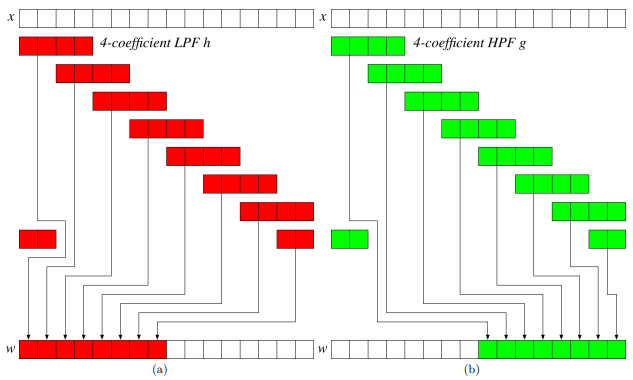
\includegraphics[width=0.7\textwidth]{imgs/waveletstep}
		\label{fig:waveletstep}
	\end{figure}
	\FloatBarrier
	\begin{figure}[h]
		\caption{Three-level wavelet transform on signal $x$ of length 16. Note that from $w_1$ to $w_2$, coefficients $H_1$ remain unchanged, while from $w_2$ to $w_3$, coefficients $H_1$ and $H_2$ remain unchanged.}
		\centering
		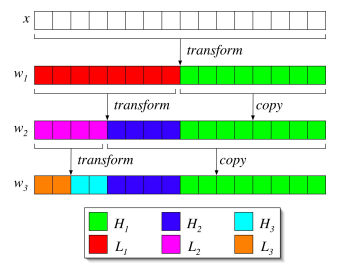
\includegraphics[width=0.7\textwidth]{imgs/three-level-DWT}
		\label{fig:3-level-DWT}
	\end{figure}
	\FloatBarrier
	\begin{figure}[h]
		\caption{One-level, two-dimensional DWT. First, the one-dimensional DWT is applied along the rows; second, the one-dimensional DWT is applied along the columns of the first-stage result, generating four sub-band regions in the transformed space: LL, LH, HL and HH.}
		\centering
		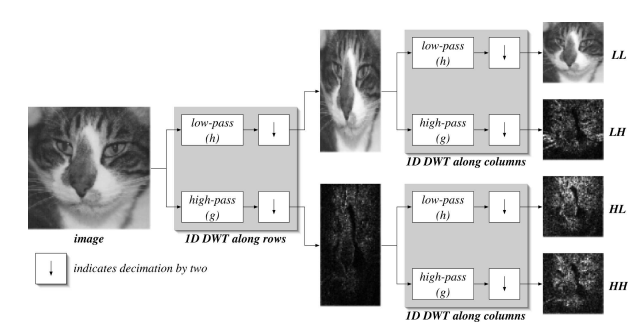
\includegraphics[width=0.9\textwidth]{imgs/2-di-wavelet}
		\label{fig:2-di-DWT}
	\end{figure}
	\FloatBarrier
	\begin{figure}[t]
		\caption{Two-dimensional wavelet transform: (left) one-level 2D DWT of sample image, and (right) threelevel 2D DWT of the same image. Note that the LH bands tend to isolate horizontal features, while the HL band tend to isolate vertical features in the image.}
		\centering
		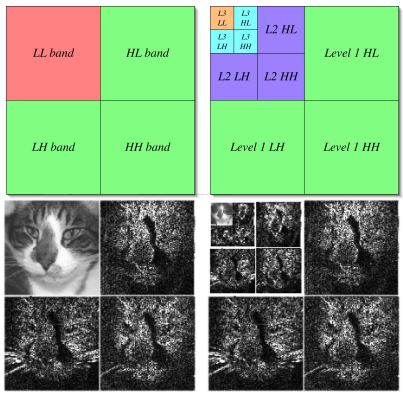
\includegraphics[width=0.8\textwidth]{imgs/multi-level-2-dwt}
		\label{fig:multi-level-2-dwt}
	\end{figure}
	\FloatBarrier
	\begin{figure}[t]
		\caption{(a) Image example, (b) construction of co-occurrence matrix (c)	matrix framework for $0^{\circ}$, (d) matrix framework for $45^{\circ}$, (e) matrix framework for $90^{\circ}$, (f) matrix framework for $135^{\circ}$}
		\centering
		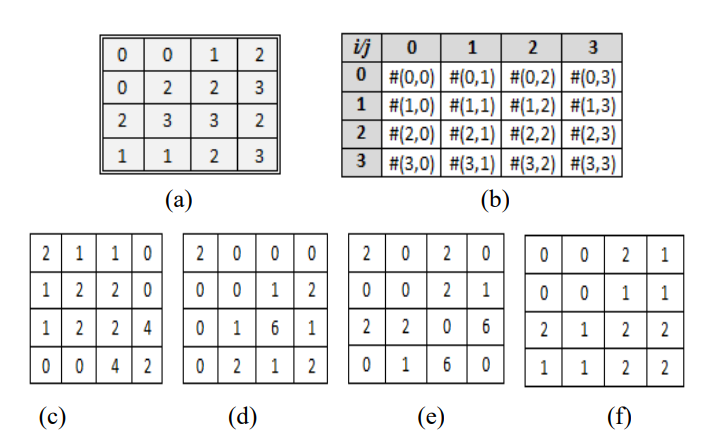
\includegraphics[width=0.8\textwidth]{imgs/glcm}
		\label{fig:glcm}
	\end{figure}
	\FloatBarrier
	\section{Table Appendix}
	\FloatBarrier
\end{document}




